%%% Ch.3: Methodology %%%
\chapter{Methods} \label{ch:method}



\section{Markov chain Monte Carlo methods}
 One common way to effectively simulate systems with a large number of degrees of freedom is to apply Monte-Carlo simulations \cite{newman1999monte}. 
 
 We apply the Metropolis Monte Carlo method based on Markov chain. The main idea is to construct Markov chain which has the given probability distribution as equilibrium distribution \eqref{partitionfunction}. In Markov chain Monte Carlo methods (often referred to as MCMC methods),  the next sample is dependent on the last accepted one.  
 
  \par For generating an appropriate random set of states according to the given probability distribution \eqref{partitionfunction}, the conditions of ergodicity and detailed balance should be placed on the Markov chain as it was proposed in \cite{doi:10.1063/1.1699114}.  
  Ergodicity means that algorithm can generate any state $u_{new}$ from any other state $u_0 $ in a finite number of steps. In physics the detailed balance means that each elementary process is in equilibrium with its reverse process. Detailed balance condition can be written as follows:
  \begin{equation}
  \label{detailedbalance}
  p_{u_0} P(u_0 \rightarrow u_{new} ) = p_{u_{new}} P( u_{new} \rightarrow u_0),
  \end{equation}
  where $P(u_0\rightarrow u_{new} )$ is the transition probability from state $u_0$ to $u_{new}$. Here, $p_{u_0},p_{u_{new}}$ are stationary Gibbs distribution probabilities: $p_{u_0} = e ^{-H(u_0)}/Z $.   Following common way, we introduce the acceptance ratio $A(u_0 \rightarrow u_{new})$ and write:
  \begin{equation*}
  P(u_0 \rightarrow u_{new}) = g(u_0 \rightarrow u_{new}) A(u_0 \rightarrow u_{new}),
  \end{equation*}
where $g(u_0  \rightarrow u_{new} )$ is the selection probability that algorithm will generate a state $u_{new}$ from an initial state $u_0$. 

\section{MCMC of three updates}
In this work, we construct Markov Chain Monte Carlo method for fixed-length chain consisting of three types of updates. We refer to them as Snake-like step, Reconnection and Wolff Cluster update. In each iteration, the algorithm chooses the update according to probabilities. We define these probabilities as $P_{local}$,$P_{reconnect}$ and $P_{Wolff}$ respectively. The sum of probabilities is always equal to one: $P_{local} + P_{reconnect} + P_{Wolff} = 1$. This algorithm was described and used to study Ising model on SAWs \cite{PhysRevE.104.054501}. 

\subsection{Snake-like algorithm}
 \begin{figure} 
	\centering
	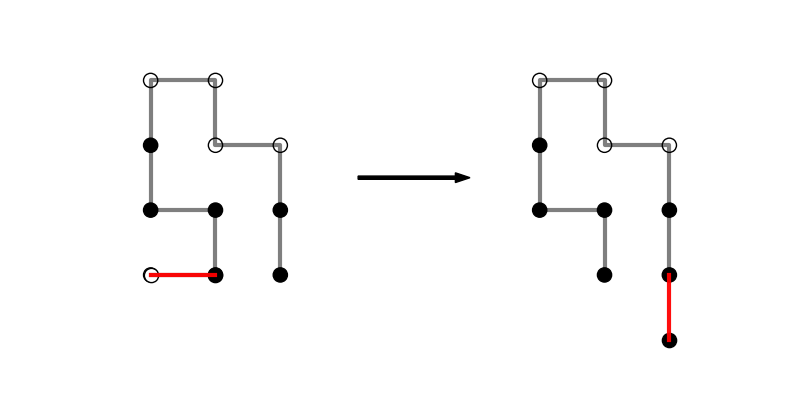
\includegraphics[scale=0.2]{Images/snakeupdate.png} 
	\captionsetup{justification=centering} \caption{ Example of snake update. }
	\label{fig:snake}
\end{figure}
This is classical method to generate SAWs which brings to mind snakes move \ref{fig:snake}  \cite{Binder2010}. The snake algorithm is a bilocal reptation update. The algorithm removes a monomer from one end and adds a monomer to the other end. Spin angle value $\theta_{new}$ and the direction in conformation are randomly generated. The direction is chosen uniformly with the probability $\frac{1}{2d}$, where $d$ is the dimensions of the lattice. The spin angle variable $\theta_{new}$ is generated uniformly $\theta_{new} \sim U(-\pi, \pi)$. The new generated state is simply accepted  according to the Metropolis rule:
\begin{equation}
\label{accratios}
A(u_0  \rightarrow u_{new} ) =  
\begin{cases}
e^{-J(E_{u_{new}}-E_{u_0})}, & \text{if $E_{u_{new}}-E_{u_0}>0$;}\\
1, & \text{otherwise}.
\end{cases}
\end{equation}

The snake update is very convenient to implement and the time and the  memory complexity $O(1)$. However, the correlation time is quite long $ \eta \sim N^2 $ and the system can be locked in the frozen states when both ends of the conformation are surrounded by $2d$ neighbors. 

\subsection{Reconnect}

 \begin{figure}[H] 
	\centering
	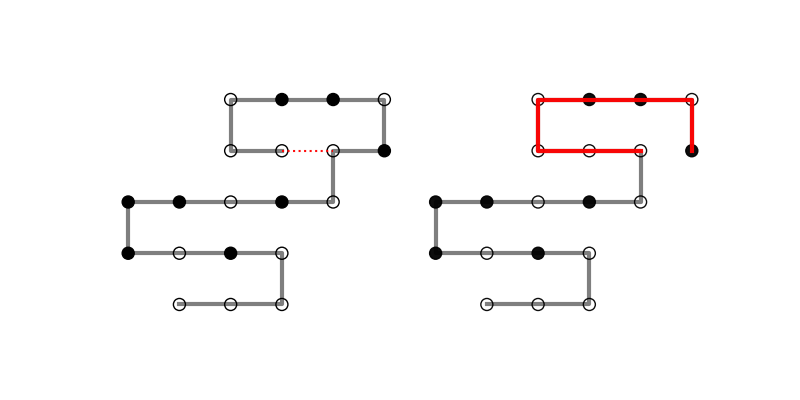
\includegraphics[scale=0.2]{Images/reconnect.png} 
	\captionsetup{justification=centering} \caption{ Example of reconnect update. }
	\label{fig:reconnect}
\end{figure}

Reconnect is a non-local update based on ideas of Worm algorithm for Ising model \ref{fig:reconnect} \cite{Worm}.   In this system update, only connections of conformation are changed. The acceptance probability is always equal to zero as the energy does not change. 

The algorithm allows system to return from frozen stated. The reconnect algorithm also allows to effectively generate conformations. The time complexity $O(N)$.  

\subsection{Wolff cluster update}
% https://math.stackexchange.com/questions/13261/how-to-get-a-reflection-vector
This is classical The Wolff algorithm for Monte Carlo simulation which we use to improve investigation of the spin configuration space  \cite{wolff}. 

The main idea of the update is to form the cluster $C$ of spins and flip its spins. The update rules should obey the detailed balance condition. We follow the classical way of cluster update implementation for XY model discussed in Ref. \cite{newman1999monte}.  

 To flip spin  using chosen direction $\vec{n}$ means to change sign of vector $ \vec{n} \vec{S_i} (\theta_i) = \vec{n}(\cos \theta_i \sin \theta_i  )$  to the opposite. 

1. Choose randomly the spin $\overrightarrow{S_{start}}$ from the chain using discrete uniform distribution. 

2. Choose the direction on the unit circle $\vec{n}$ using uniform distribution $ U(-\pi, \pi)$.

3. Update the chosen monomer $\overrightarrow{S_{start}}$. To do it, we need to change sign of $ \vec{n}  \overrightarrow{S_{start}} $ to the opposite. This action is the subtraction the reflected  $\vec{n}$  from $ \overrightarrow{S_{start}} $. Therefore, the flip is implemented as following: $\overrightarrow{S_{start}} := \overrightarrow{S_{start}} - 2 \times ( \overrightarrow{S_{start}} \vec{n}) \times \vec{n}$. We add this flipped spin to the cluster $C$.

4. Now it is time to grow the cluster $C$. Visit all the lattice neighbors $\overrightarrow{S_{i}}$ of $\overrightarrow{S_{start}}$ and flip them if the signs of the directions $ \vec{n} \overrightarrow{S_{i}}$  and $ \vec{n} \overrightarrow{S_{start}}$ are the same. Flip the visited cite and add them to the cluster: $\overrightarrow{S_{i}} : = \overrightarrow{S_{i}} - 2 \times ( \overrightarrow{S_{i}} \vec{n}) \times \vec{n}$. 

5. Now continue to visit neighbors of spins from cluster $C$ and flip spins according the same procedure as described in previous step. 

The algorithm effectively sample spin configurations and keep the conformation fixed. The time complexity $O(1)$. 
 


